\section{Containerization Software}
Containerization software is used to isolate processes running on a host from one another.
A process in a container sees a different part of the host system then processes outside of the container. A process inside a container sees a different file system, network interfaces and users than processes outside of the container. Processes inside the container can only see other processes inside the container.

\begin{figure}[ht]
    \begin{subfigure}{.45\textwidth}
        \centering
        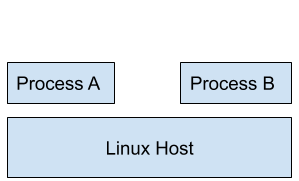
\includegraphics[width=.8\linewidth]{resources/images/no-containers.png}
        \caption{Two processes}
    \end{subfigure}
    \begin{subfigure}{.45\textwidth}
        \centering
        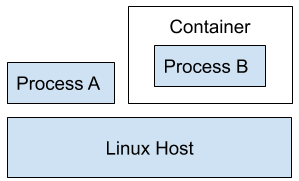
\includegraphics[width=.8\linewidth]{resources/images/container.png}
        \caption{One process in a container}
    \end{subfigure}
    \caption{}
\end{figure}

If we look at the above example, we see two scenarios. The first is the default way to run processes. The operating system starts processes that can communicate with one another. Their view on the file system is the same.
In the second scenario one of the processes runs inside a container. These processes cannot communicate with one another. If Process A looks at the files in \lstinline{/tmp}, it accesses a different part of the file system than if Process B looks at the files in \lstinline{/tmp}. Process B can not even see that Process A exists.

\hfill

Process A and Process B see such a different part of the host system that to Process B it looks like it is running on a whole separate system.

\subsection{Why use containers?}

Containers can be made into easily deployable packages (called images). These images only contain the necessary files for specific software to be run. Other files, libraries and binaries are shared between the host operating system (the system running the container). This allows developers to create lightweight software packages containing only the necessary dependencies.

\hfill

Containers also make it possible to run multiple versions of the same software on one host. Each container can contain a specific version and all the containers run on the same host. Because the containers are isolated from each other, their incompatible dependencies are not a problem.

\hfill

For example, someone who wants to run an instance of Wordpress\footnote{A very popular content management system to build websites with.} does not need to install all the Wordpress dependencies. They only need to download the container that the Wordpress developers created, which includes all the necessary dependencies.

Similarly, if they want to move the Wordpress instance from one host to the other, they just have to copy over their database and run the image on the new host. Even if the new host is a completely different operating system.

If they want to test a newer version of Wordpress on the same host, they only have to run the different container on the same host. The incompatible dependencies of the two Wordpress instances are not a problem, because they see another part of the file system and do not even see each other's process.

\hfill

This ease of use makes containerization very popular in software development, maintenance and deployment.

\pagebreak

\subsubsection{Virtualization}
Virtualization is an older similar technique to isolate software. In virtualization, a whole system is simulated in top of the host (called the hypervisor). This new virtual machine is called a guest. The guest and the host do not share any system resources. This has some advantages. For example, it allows running a completely different operating system as guest (e.g. Windows guest run on a Linux host).

\begin{figure}[ht]
    \begin{subfigure}{.45\textwidth}
        \centering
        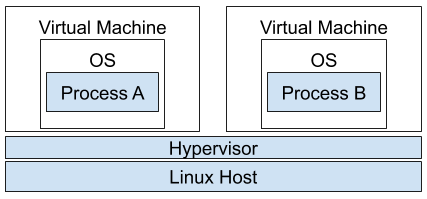
\includegraphics[width=.8\linewidth]{resources/images/virtual-machines.png}
        \caption{Virtual machines}
    \end{subfigure}
    \begin{subfigure}{.45\textwidth}
        \centering
        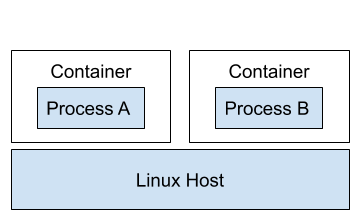
\includegraphics[width=.8\linewidth]{resources/images/containers.png}
        \caption{Containers}
    \end{subfigure}
    \caption{}
\end{figure}

Because containerization software shares many resources with the host, it is a lot faster and more flexible than virtualization. Where virtualization needs to start a whole new operating system, containerization only needs to start a single process.

\subsubsection{Containers for security}

Isolation reduces risk, because it separates processes. If one process is compromised it cannot reach another process. If a process in a container is compromised, it cannot reach sensitive files of the host. This clearly add security value.

\hfill

It should be noted, however, that containerization is a lot more risky than virtualization, because containers run using the same kernel and resources as the host. For example, this means that a kernel exploit run inside a container is just as dangerous as the same exploit run directly on the host, because the target (the kernel) is the same.
